\appendix
The mapping of the physics tendencies from the physics grid to the GLL grid is done with tensor-cubic Lagrange interpolation. The elements of the cubed-sphere in SE are created from an equi-angular gnomonic projection. Consider one element $(\alpha,\beta) \in \left[ \alpha^{(elem)}_1,\alpha^{(elem)}_2 \right]\times \left[ \beta^{(elem)}_1,\beta^{(elem)}_2\right]$, where $(\alpha,\beta)$ are central angle coordinates and $\alpha^{(elem)}_1$ and $\alpha^{(elem)}_2$ are the minimum and maximum central angles in the $\alpha$-coordinate direction, respectively, and similarly for $beta$. Let $\Delta \alpha^{(elem)}=\alpha^{(elem)}_2-\alpha^{(elem)}_1$ and $\Delta \beta^{(elem)}=\beta^{(elem)}_2-\beta^{(elem)}_1$. The physics grid cell central angle centers are located at
\begin{multline}
(\alpha^{(pg)}_i,\beta^{(pg)}_j)= \Big[ \alpha^{(elem)}_1+\left(i-\tfrac{1}{2}\right) \Delta \alpha^{(pg)},\\
                                      \beta^{(elem)}_1+\left(j-\tfrac{1}{2}\right) \Delta \beta^{(pg)}\Big],
\end{multline}
where $\Delta \alpha^{(pg)}=\Delta \beta^{(pg)}=\frac{\Delta \alpha^{(elem)}}{pg}=\frac{\Delta \beta^{(elem)}}{pg}$. The interpolation is performed in central-angle coordinates using tensor product cubic interpolation. For elements located on a cubed-sphere edge or corner the coordinate system for neighboring elements may be on a different panel. To take into account this coordinate change the central angle locations of physics grid cell centers located on other panels are transformed to the coordinate system of the panel the element in question is located on \cite[the transformations are given in, e.g.,  ][]{NTL2005MWRb}. An illustration is given in Figure \ref{fig:mapping} for an element located in the lower left corner of a panel. The element in question is $(\xi,\chi)\in (-1,1)^2$ where, for simplicity, we have transformed the element coordinates into normalized coordinates $(\xi,\chi) = \left( \frac{ 2\left(\alpha^{(pg)}-\alpha^{(elem)}_1\right)}{\Delta \alpha^{(elem)}}-1,\frac{2\left( \beta^{(pg)}-\beta^{(elem)}_1\right)}{\Delta \beta^{(elem)}}-1\right)$; also used internally in the SE dynamical \citep[see, e.g., section 3.3 in ][]{LetAl2017MWR}. The GLL points are located at -1,$-\sqrt{5}/5$, $\sqrt{5}/5$, and 1 in each coordinate direction. Near the edges/corners of an element cubic extrapolation is used if the centered stencil expands beyond the panel.

\begin{figure}[t]
\noindent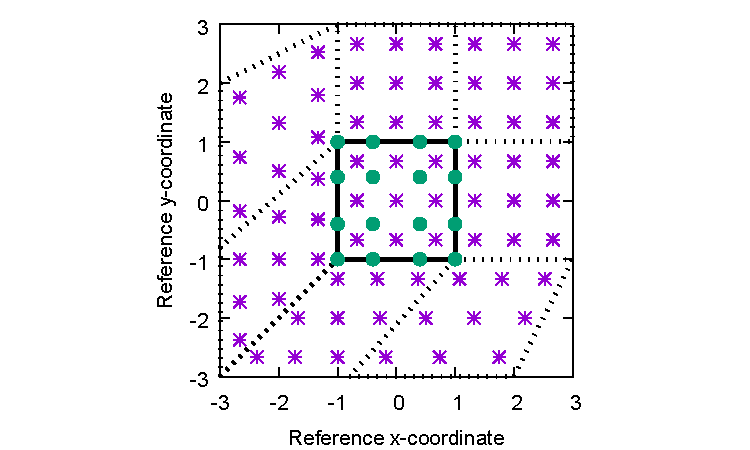
\includegraphics[width=19pc,angle=0]{figs/mapping/mapping.pdf}\\
\caption{Schematic of the coordinate system in which the dimensionally split cubic Lagrange interpolation is computed.  The physics grid centers are marked with asterisks and the GLL points, we are interpolating to, with solid filled circles. The element in which the GLL points are located is  bounded by  thick black lines and located in the lower left corner of a panel. The stippled lines mark the boundaries of the remaining elements. For simplicity we are using the normalized coordinate centered at the element on which the GLL points we are interpolating to are located. Note that the coordinates for points on neighboring panels (using a different local coordinate system) must be transformed to the coordinate system of the element in question.}
\label{fig:mapping}
\end{figure}
